\documentclass{article}

\usepackage{amsmath}
\usepackage{amsfonts}
\usepackage{graphicx}
\usepackage[section]{placeins}
\usepackage[a4paper, total={6.5in, 10in}]{geometry}
\usepackage{listings}

\usepackage{xcolor}
\usepackage{pagecolor}
\pagecolor{black}
\color{white}

\lstset{
    breaklines=true,
    tabsize=4,
    basicstyle=\ttfamily,
    literate={\ \ }{{\ }}1
}

\title{-}
\author{-}

\begin{document}

\begin{center}

	\Large\bfseries
	Methods for recognizing dimensions of rectangular panels and laying panels on planar surfaces

\end{center}

\section{Introduction}

The problem originated from the task of generating rectangular tile layout for KSA Pavilion. It involves two parts: 1. For convenience of users and recycling process, an algorithm is needed to recognize the dimensions of given tiles (Figure \ref{recognition}). 2. Given surfaces and numeric desciption of panel options, fill surfaces with panels in a random way with optional gradient effect without leaving gaps. (Figure \ref{overview}).

\begin{figure}[hbt!]
	\centering
	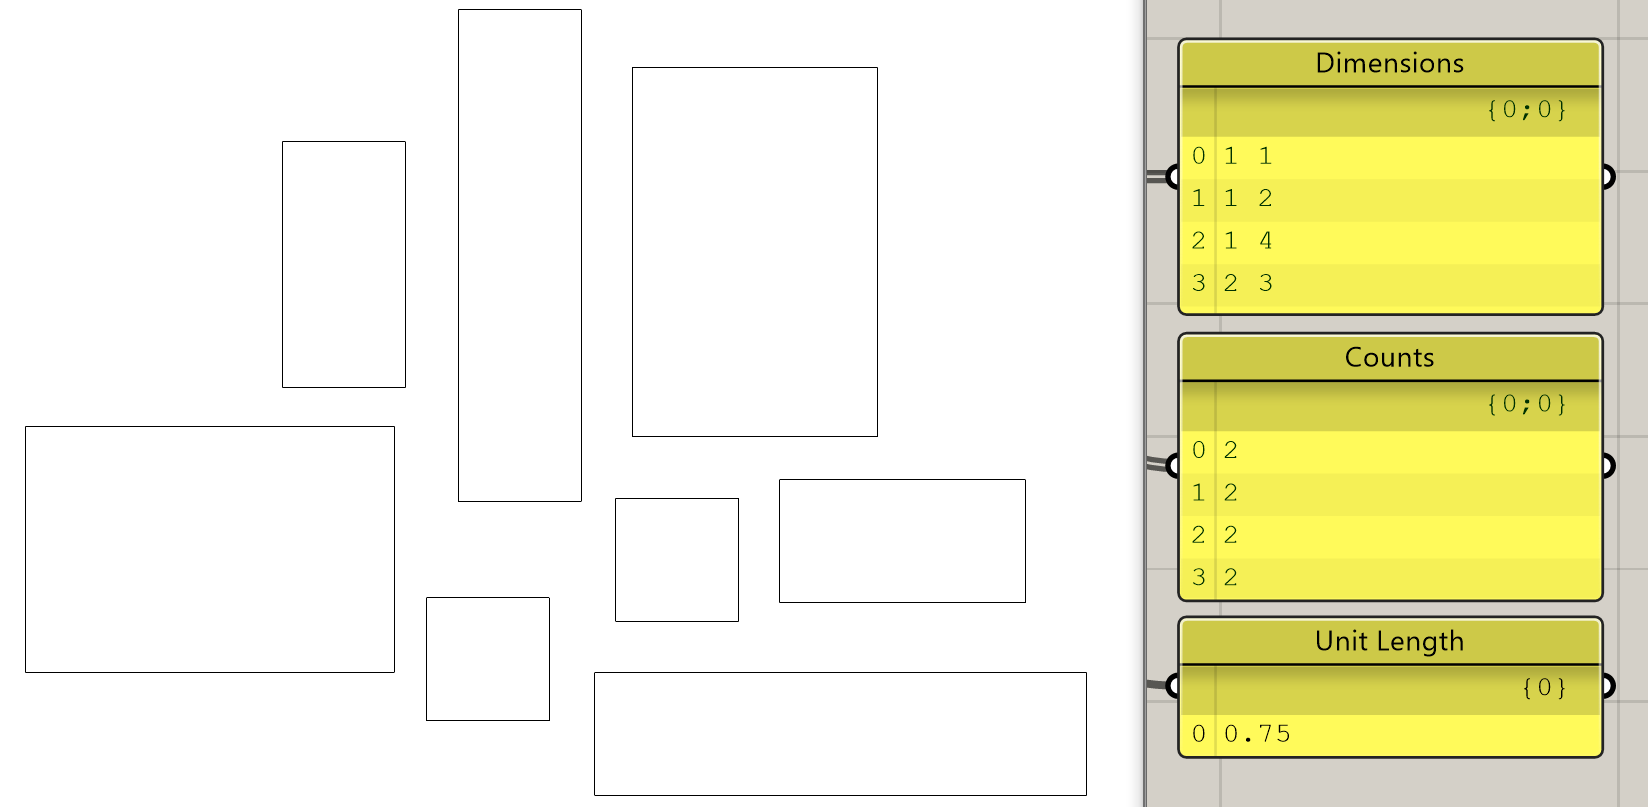
\includegraphics[width=0.75\textwidth]{Figures/Recognition.png}
	\caption{
        Example result of dimension recognition
    }
	\label{recognition}
\end{figure}

\begin{figure}[hbt!]
	\centering
	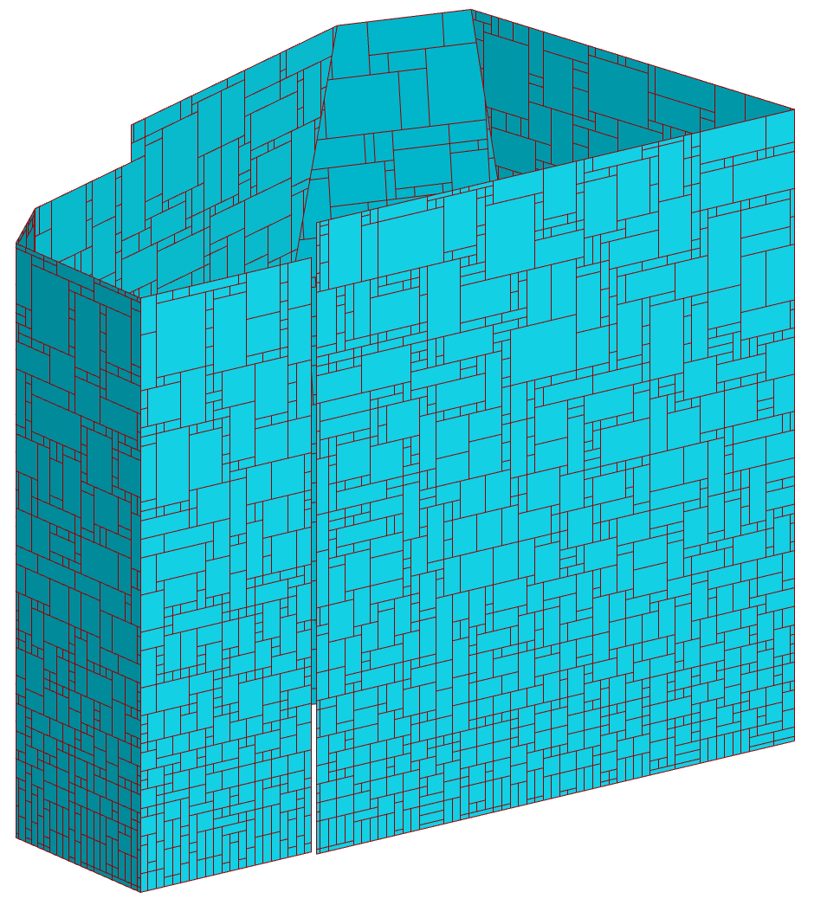
\includegraphics[width=0.4\textwidth]{Figures/Overview.png}
	\caption{Example of gradient "Orthogonal" tiling of KSA Pavilion}
	\label{overview}
\end{figure}

\FloatBarrier

\section{Overview of the algorithm}

The algorithm improved the running speed of placing rectangular tiles by converting both given options and target surfaces to numeric and rasterized descriptions. The algorithm is internalized in the GH script so that feeding curves and surfaces in Rhino is sufficient for running the whole process.

\subsection{Abstracting tile options}

In the first part, numeric description will be extracted from tile options in form of Rhino curves (denoting outlines of tiles). (Figure \ref{num}) In this way, the designers can simply draw options in Rhino. Also, since the output of tiling algorithm is also a group of outlines in format of Rhino curves, having this algorithm can quickly recognize the dimensions and count the numbers for reusing tiles.

\begin{figure}[hbt!]
	\centering
	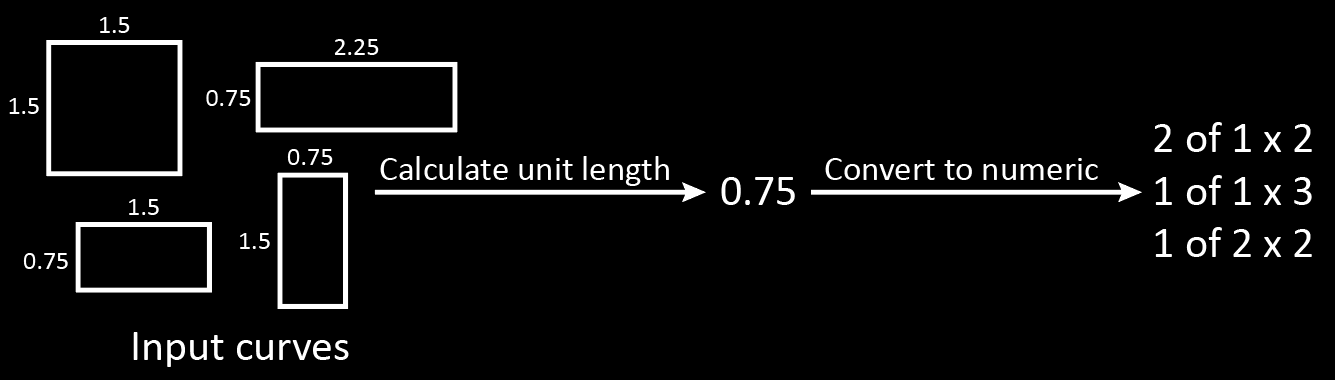
\includegraphics[width=0.75\textwidth]{Figures/Numeric.png}
	\caption{Sample of numeric description of options}
	\label{num}
\end{figure}

\subsection{Rasterizing surfaces}

The surfaces to be tiled will be converted to point grid by grasshopper components. Then, a two dimentional boolean array will be constructed accordingly for the algorithm, where true denotes available (uncovered) positions and false denotes occupied (either outside the shape or have already been covered by earlier tiles) positions. (Figure \ref{rast})

\begin{figure}[hbt!]
	\centering
	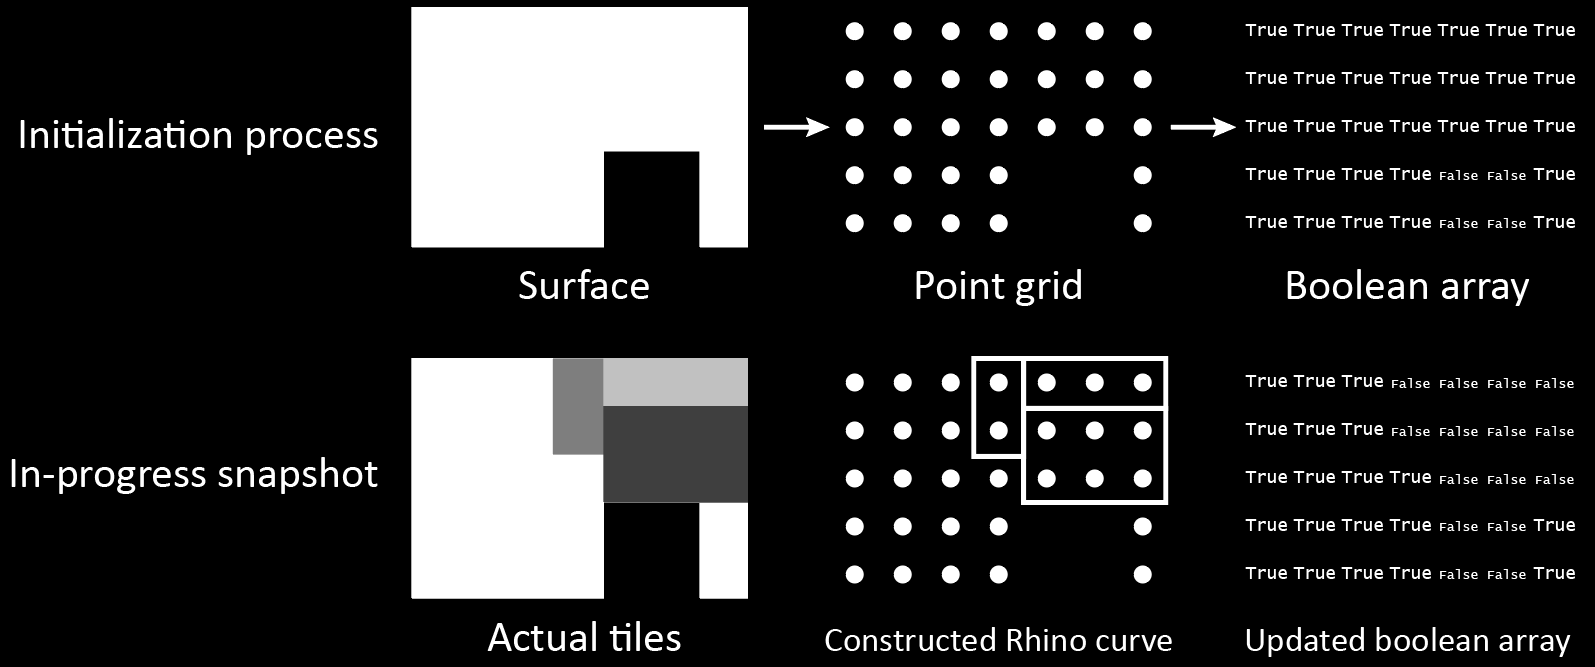
\includegraphics[width=0.9\textwidth]{Figures/Rasterization.png}
	\caption{Sample of rasterization process}
	\label{rast}
\end{figure}

\FloatBarrier

\section{Overview of implementation}

The actual implementation of the algorithms assumes all input and output to be on XY plane aligning with axes in convenience of future application in different scenarios. The current script includes the following steps:

\textbf{1.} Extract tile dimension options and (opitionally) specify numbers or percentages of each type as numeric descriptions.

\textbf{2.} Orient given surfaces to XY plane and generate point grid along X/Y axes.

\textbf{3.} Convert point grid to boolean array.

\textbf{4.} Initialize position queue with shuffled order.

\textbf{5.} Attempt to place tiles from largest to smallest in available positions in the shuffled order.

\textbf{6.} Construct curves.

\textbf{7.} Orient curves back to surfaces.

Please see the diagram showing how they are involved in KSA Pavilion (Figure \ref{diagram}).

\begin{figure}[hbt!]
	\centering
	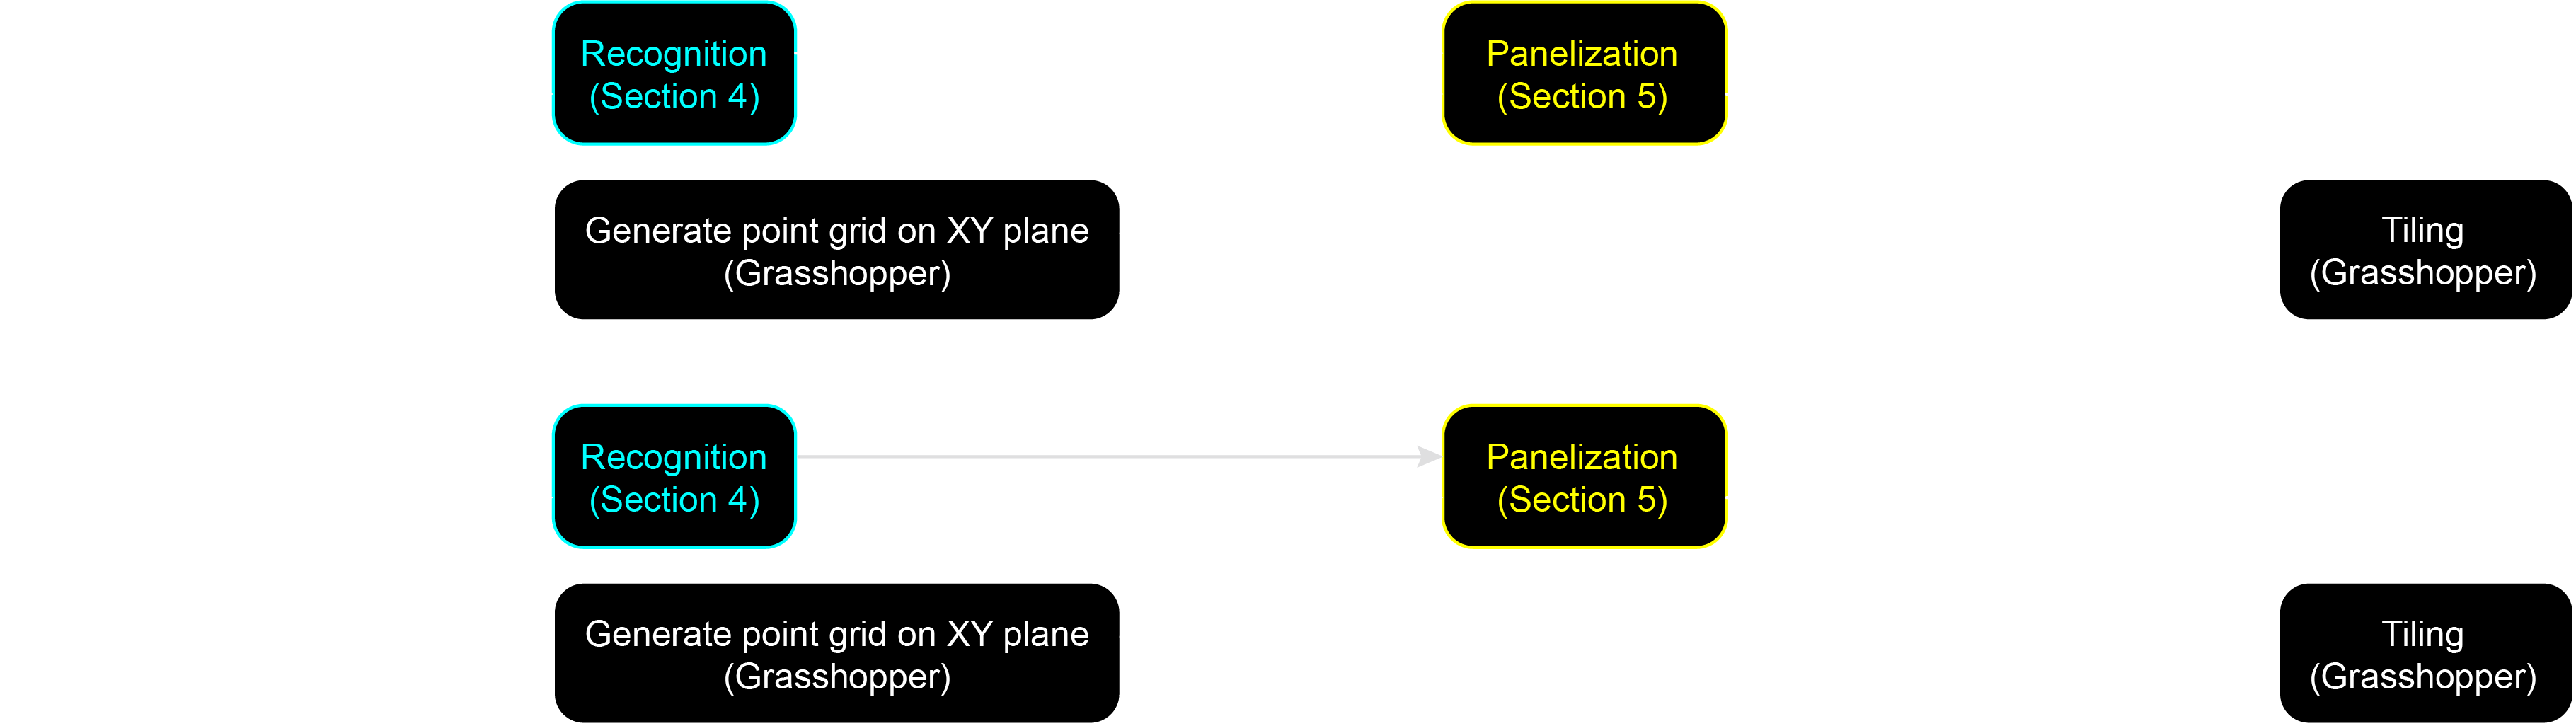
\includegraphics[width=1\textwidth]{Figures/Diagram.png}
	\caption{Diagram of components used in KSA Pavilion project}
	\label{diagram}
\end{figure}

\section{Recognition}

The unit length of the tiles is the greatest common divisor (GCD) of their widths and heights. The only extra part to pay attention is to deal with non-integer dimensions. Below is the detailed steps:

Denoting the collection of bounding boxes of each panel as B.

\textbf{1.} Extract the set of lengths from bounding boxes' width and length.

\textbf{2.} Scale all numbers by $10^n$ if they are decimal numbers accurate to $n$ decimal places.

\textbf{3.} Calculate GCD of all numbers. Pseudo code:

\begin{lstlisting}[language=Python]
	//arr contains all the integers GCD to be calculated
	result = arr[0]
	for i in range(len(arr)):
		result = gcd(result, arr[i])
\end{lstlisting}

Note: GCD of two numbers can be calculate with \href{https://en.wikipedia.org/wiki/Euclidean_algorithm}{Euclidean algorithm}. Pseudo code:

\begin{lstlisting}[language=Python]
	//Calculate GCD of a and b
	def gcd(a, b):
		if b == 0:
			return a
		return gcd(b, a % b)
\end{lstlisting}

\textbf{4.} Divide all dimensions by GCD to get normalized dimensions.

\textbf{5.} Scale GCD by $1/10^n$ to get the unit length.

\section{Panelization}

The main idea of this algorithm is to use 2D array for placing panels, instead of checking whether the panel fits a place through geometrically testing intersections. It is convenient whether the user would like to feed in Rhino curves or values to describe the panel options.

A queue of positions in a pregenerated random order is used instead of randomly picking positions ensures all positions are filled. If a panel doesn't fit a position, it will never fit later. Therefore, for each tile option, iterating through all available positions once is sufficient, and positions not fitting can be put to the end of the queue for smaller options.

\subsection{Steps}

Preprocess: Convert given surfaces to point grid aligning with XY axes with same unit length as panels. This is achieved by Grasshopper. Besides, add infinite number of 1x1 tiles to ensure all gaps to be filled.

\textbf{1.} Convert given point grid to 2D array, where boolean value \lstinline{map[i][j]} denotes whether position $i,j$ has been occupied.

\textbf{2.} Create a queue and enqueue all available positions in a random order.

Note 1: A random permutation of a sequence can be generated in $\mathcal{O}(n)$. Pseudo code:

\begin{lstlisting}[language=Python]
	//arr contains the sequence to be shuffled
	for i in range(n - 2):
		j = i + random_integer(n - i)
		swap(arr[i], arr[j])
\end{lstlisting}

where \lstinline{random_integer(n)} randomly pick an integer $0 \leq x < n$.

Note 2: In KSA Pavilion project, the extra step to achieve a gradient effect is to generate the random permutation non-uniformly with a custom \lstinline{random_integer} method. Pseudo code:

\begin{lstlisting}[language=Python]
	def random_integer(n, grad)
		pick = random() * n ** grad / (grad + 1)
		return int(n - (pick * (grad + 1)) ** (1 / (grad + 1)))
\end{lstlisting}

where parameter \lstinline{grad} controls how much gradient effect and \lstinline{random()} randomly pick a floating number between 0 and 1. Note that using integer for \lstinline{pick} will result in unsmooth distribution.

\textbf{3.} From largest to smallest, attempt to lay all panels to the 2D space. Pseudo code:

\begin{lstlisting}[language=Python]
	for option in options:
		i = 0
		position_count = size(queue)
		while i < position_count and option.remaining > 0:
			position = queue.Dequeue()
			if map[position.x][position.y] and fit(option, position):
				option.remaining--
				construct outline curve
				update map
			else:
				queue.Enqueue(position)
			i++
\end{lstlisting}

where \lstinline{map} is the boolean array mentioned above, and each \lstinline{option} object describes the widthand height of a tile option and the remaining number of such tile (if tiling with limited amount of tiles).

\section{Notes}

\subsection{Potential Failure in Recognition}

Since dimensions are extracted by \lstinline{BoundingBox.Max - BoundingBox.Min}, There's chance for this to fail due to accuracy of floating point representation, for example getting 7499 instead of 7500 for scaled dimensions.

If the calculation result of unit length is 1 or $10^{-n}$ (for example 0.01) but the tiles don't appear to have such unit length, the algorithm may have failed (got GCD = 1). Do check the result before proceeding, since a wrongly small unit length will generate dense point grid and large boolean array.

\subsection{Notes for Panelization}

Currently the script doesn't automatically recognize unit length of point grid (it should be easy to achieve with GCD algorithm as well). So make sure to feed the correct unit length (for example directly from recognition part) to both point grid generator and panelization script, otherwise some weird results may be produced. It takes ~10 seconds to panelize the whole pavilion (~10000 panels), therefore excessively long time may indicate an error.

Since the algorithm only guarantees all points in grid to be coverd, the result of panelization also depends on whether the point grid is generated correctly (or meet the expectation), especially for non-rectangular surfaces. Trapezoid walls exist in KSA pavilion (Figure \ref{trapeziod}). Therefore, extra care is taken in point grid generator to make sure the result always covers 

\begin{figure}[hbt!]
	\centering
	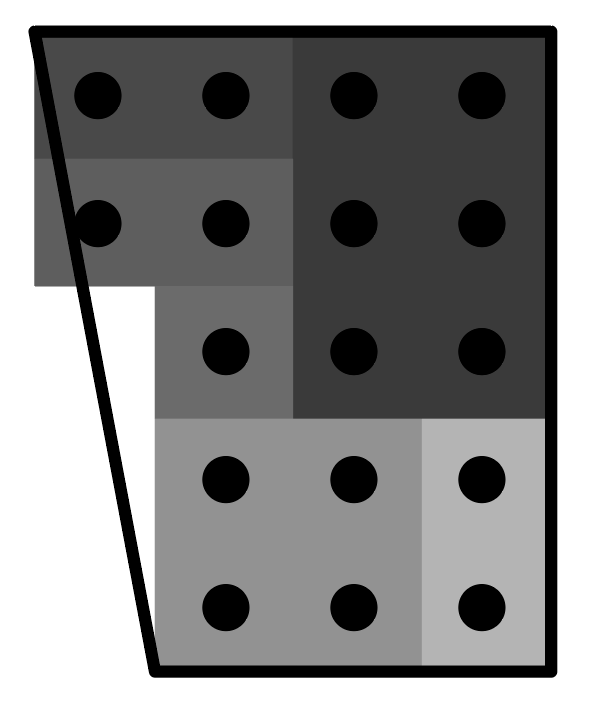
\includegraphics[width=0.2\textwidth]{Figures/BadGrid.png}
	\caption{Example point grid where a small part of the trapezoid cannot be covered by panels}
	\label{trapeziod}
\end{figure}

\FloatBarrier

\subsection{Limitations}

Due to the nature of rasterization process, the introduced algorithms can only be applied to scenarios with following characteristics: 1. Panels are rectangular; 2. The widths and heights of panels are multiplication of a fix number (i.e. a reasonable GCD exists).

\end{document}